\subsection{Investimento fase di Analisi}

\subsubsection{Divisione oraria}
La seguente tabella rappresenta la distribuzione oraria dei ruoli per ogni componente del gruppo:
{

	\rowcolors{2}{\evenRowColor}{\oddRowColor}
\renewcommand{\arraystretch}{2}
\begin{longtable}[h!] { C{3.3cm} C{1cm} C{1cm} C{1cm} C{1cm} C{1cm} C{1cm} C{2cm}}
\caption{Tabella della divisione oraria di Analisi}	\\
\rowcolor{\primaryColor}

\textcolor{\secondaryColor}{\textbf{Membro del gruppo}} & 
\textcolor{\secondaryColor}{\textbf{RE}} & 
\textcolor{\secondaryColor}{\textbf{AM}} & 
\textcolor{\secondaryColor}{\textbf{AN}} & 
\textcolor{\secondaryColor}{\textbf{PT}} & 
\textcolor{\secondaryColor}{\textbf{PR}} & 
\textcolor{\secondaryColor}{\textbf{VE}} & 
\textcolor{\secondaryColor}{\textbf{Ore complessive}}\\	
\endhead
\AW{}                     &  - &  - &  14 & - & - & 14 & 28 \\
\AT{}                     &  - &  10 & 10 & - & - & 8 & 28 \\
\AD{}                     &  - &  - &  14 & - & - & 15 & 29 \\
\EC{}                     &  - &  10 & 10 & - & - & 8 & 27 \\
\EM{}                     &  17 &  - & 7 & - & - & 8 & 32 \\
\FP{}                     &  - &  15 & 10 & - & - & 9 & 34 \\
\GG{}                     & 18 &  - &  7 & - & - & 8 & 33 \\
\textbf{Ore totali ruolo} & 35 & 35 & 71 & - & - & 70 & 211 \\

\end{longtable}
}
% Responsabile color=blue, Amministratore color=yellow, Analista color=red, Progettista color=green, Programmatore color=grigetto, Verificatore color=orange  [ybar, fill=] blue, yellow, red, green, grigetto, orange
\begin{figure}[h!]
	\caption{Istogramma relativo la suddivisione delle ore preventivate nella fase di analisi}
	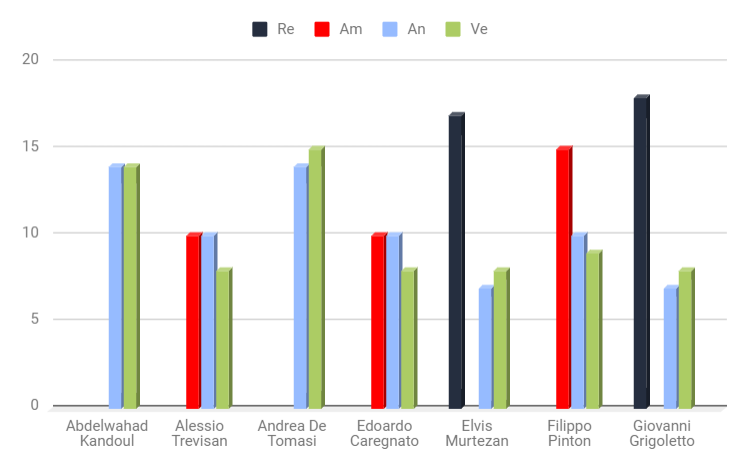
\includegraphics[width=1\textwidth]{./src/Preventivo/src/img/IstoAnalisi.png}
\end{figure}
%\begin{center}
%	\pgfplotsset{width=15.4cm, height=8.5cm}
%	\begin{tikzpicture}
%		\begin{axis}[
%			ybar stacked,
%			bar width=20pt,
%			legend style={
%				at={(0.5,-0.15)},
%				anchor=north,
%				legend columns=-1
%			},
%			symbolic x coords={Abdelwahad, Alessio, Andrea, Edoardo, Elvis, Filippo, Giovanni},
%			xtick=data
%		]
%			\legend{Responsabile, Amministratore, Analista, Progettista, Programmatore, Verificatore}
			% Responsabile
%			\addplot [ybar, fill=blue] coordinates {\ColonnaIstogramma{0}{0}{0}{0}{17}{0}{18}};
			% Amministratore
%			\addplot [ybar, fill=yellow] coordinates {\ColonnaIstogramma{0}{10}{0}{10}{0}{15}{0}};
			% Analista
%			\addplot [ybar, fill=red] coordinates {\ColonnaIstogramma{14}{10}{14}{10}{7}{10}{7}};
			% Progettista
%			\addplot [ybar, fill=green] coordinates {\ColonnaIstogramma{0}{0}{0}{0}{0}{0}{0}};
			% Programmatore
%			\addplot [ybar, fill=pink] coordinates {\ColonnaIstogramma{0}{0}{0}{0}{0}{0}{0}};
			% Verificatore
%			\addplot [ybar, fill=orange] coordinates {\ColonnaIstogramma{14}{8}{15}{8}{8}{9}{8}};
%		\end{axis}
%	\end{tikzpicture}
%\end{center}
\clearpage

\subsubsection{Costo risultante}
La seguente tabella rappresenta per ogni ruolo le ore totali investite ed il corrispondente costo in euro:
{
\rowcolors{2}{\evenRowColor}{\oddRowColor}
\renewcommand{\arraystretch}{2}
\begin{longtable}{ C{3cm} C{2cm} C{4cm}}
\caption{Tabella del costo risultante di analisi}\\
\rowcolor{\primaryColor}

\textcolor{\secondaryColor}{\textbf{Ruolo}} & 
\textcolor{\secondaryColor}{\textbf{Totale ore}} & 
\textcolor{\secondaryColor}{\textbf{Costo ruolo (in \euro{})}}\\	
\endhead

Responsabile    &  35 &  1050 \\
Amministratore  &  35 &  700 \\
Analista        &  71 & 1775 \\
Progettista     &   - &  - \\
Programmatore   &   - &  - \\
Verificatore    &  70 & 1050 \\
\textbf{Totale} & 211 & 4575 \\
		
\end{longtable}
}

\begin{figure}[h!]
	\caption{Areogramma relativo la suddivisione oraria per i diversi ruoli nella fase di analisi}
    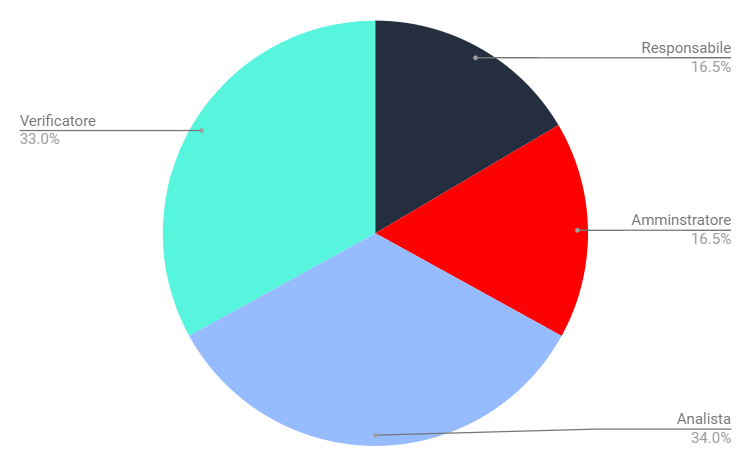
\includegraphics[width=1\textwidth]{./src/Preventivo/src/img/TortaAnalisi.png}    
\end{figure}


%La quantità di ore totali investite per ciascun ruolo viene rappresentata nel seguente areogramma:
%\begin{center}
%	\pgfplotsset{width=17cm, height=8.5cm}
%	\begin{tikzpicture}
%		\pie[rotate = 180, color={blue, yellow, red, orange}] {
%			17/Responsabile,
%			17/Amministratore,
%			33/Analista,
%			33/Verificatore
%		}
%	\end{tikzpicture}
%\end{center}
